\documentclass{article}
\usepackage{amsmath, amsthm, amssymb, amsfonts, mathtools,enumitem, stmaryrd,physics, cancel, tikz-cd, graphicx, float, booktabs, xurl}
\usetikzlibrary{arrows}
\usepackage{geometry}
    \geometry{
        a4paper,
        left = 40mm,
        top = 20mm,
        right = 40mm,
        bottom = 30mm
    }
\setlength{\parindent}{0pt}

\theoremstyle{definition}
\newtheorem{problem}{Problem}
\newtheorem{solution}{Solution}
\newtheorem*{example}{Example}
\newtheorem*{exercise}{Exercise}
\newtheorem*{definition}{Definition}
\newtheorem{theorem}{Theorem}
\newtheorem*{theorem*}{Theorem}
\newtheorem{proposition}[theorem]{Proposition}
\newtheorem*{proposition*}{Proposition}
\newtheorem{lemma}[theorem]{Lemma}
\newtheorem*{lemma*}{Lemma}
\newtheorem{corollary}[theorem]{Corollary}
\newtheorem*{corollary*}{Corollary}
\newtheorem*{remark}{Remark}

\title{M633 Algebraic Varities I}
\author{Thanic Nur Samin}
\date{}

\begin{document}
    \maketitle

    \section*{Monday, 8/25/2025}
    
    Textbook: The Rising Sea.
    
    Link: \url{https://math.stanford.edu/~vakil/216blog/FOAGjul2724public.pdf}

    Office Hours: Wednesdays 3-4, Fridays 1-2

    It's basically an introduction to the scheme point of view for algebraic geometry.

    Grothendieck POV: if we get the definitions right, hard problems will become easier. We are trying to get the definition here.

    \section*{Motivation / A Pseudo History}

    Let \(X\) be a topological space (Compact, Hausdorff).

    \(C(X)=\) ring of real-valued continuous functions.

    Question: What are the maximal ideals of \(C(X)\)?

    Fact: TFAE: given a ring \(A\),

    \begin{enumerate}[label=\roman*)]
        \item \(I\) is maximal among proper ideals of \(A\)
        \item \(A / I\) is a field
        \item There exists a surjective homomorphism from \(A\) to a field \(F\), \(\phi : A \to F\) such that \(I = \ker \phi\)  
    \end{enumerate} 

    If \(x_0\in X\), we have the ring homomorphism \(\operatorname{eval}_{x_0}: f \mapsto f(x_0)\).

    This is an \(\mathbb{R}\)-linear map.

    This is also obviously surjective.

    Thus, \(\ker \operatorname{eval}_{x_0} = \left\{ f\in C(x) \mid f(x_0) = 0 \right\}\). This is a maximal ideal. In fact,

    \begin{theorem}
        All maximal ideals of \(C(X)\) are of the form \(\ker \operatorname{eval}_{x_0}\).
    \end{theorem}

    \begin{proof}
        Suppose not. Let \(\phi : C(X) \to F\) be a surjective homomorphism to a field, and let \((f_1, f_2, f_3, \cdots) = \ker \phi\).
        
        If \(\ker \phi \neq \ker \operatorname{eval}_{x_0} \implies \exists f_{x_0}\in \ker \phi\) such that \(f_{x_0}(x_0)\neq 0\). This is true for each point \(x_0\in X\).

        Therefore, \(f_{x_0}(x)\neq 0\) for all \(x\in U_{x_0}\) where \(U_{x_0}\) is an open neighborhood of \(x_0\).

        Since \(X\) is compact, there is \(x_1, \cdots , x_n \in X\) so that \(U_{x_j}\) cover \(x\).

        \(f_1, \cdots , f_n \in \ker \phi\) such that \(f_i(x) \neq 0 \forall x\in U_{x_i}\).

        Then \(f(x) \coloneqq \sum_{i} f_i^2(x) > 0\) for all \(x\in X\). Then \(\frac{1}{f}\in C(X) \implies 1\in \ker \phi\). Contradiction!  
    \end{proof}

    Given \(f\in C(X)\) define \(Z(f) = f ^{-1} (0)\). This is a closed subset of \(X\).
    
    We can do abuse of notation and say \(X = \operatorname{Max}(C(X))\).

    Then \(Z(f) = \left\{ \mathfrak{m} \in \operatorname{Max} (C(X)) \mid f\in \mathfrak{m} \right\} \) 

    Then, \(Z(f)^c\) open in \(X\)

    \(= \left\{ \mathfrak{m} \in \operatorname{Max} (C(X)) \mid f\notin \mathfrak{m} \right\} \) 

    We have successfully turned a topological space into a ring.

    If we have \(X \xrightarrow{cont} Y\) we have \(C(Y) \to C(X)\).

    Instead of arbitrary topological spaces, now we focus on \(\mathbb{C}^n\).

    Lets look at polynomials \(\mathbb{C}^n \to \mathbb{C}\).

    Ring of polynomial functions is \(\mathbb{C} [x_1, \cdots , x_n]\).

    \begin{theorem}
        [Weak Hilbert Nullstellensatz] Maximal ideals of this ring are exactly the kernels of evaluation maps at points \((a_1, \cdots , a_n) \in \mathbb{C}^n\).
    \end{theorem}

    Note that \(x_1 - a_1, \cdots , x_n - a_n\in \ker \operatorname{eval}_{(a_1, \cdots , a_n)}\). In fact, \(\ker \operatorname{eval}_{(a_1, \cdots , a_n)} = (x_1 - a_1, \cdots , x_n - a_n)\).

    \begin{proof}
        WLOG \(a_1 = \cdots = a_n = 0\). Then \(\ker \operatorname{eval}_{(0,\cdots ,0)}\) are exactly the polynomial with no constant term, which is exactly \((x_1, \cdots , x_n)\).
    \end{proof}

    Now we prove weak Nullstellensatz.

    \begin{proof}
        Let \(\mathfrak{m} \subset \mathbb{C} [x_1, \cdots , x_n]\) be a maximal ideal. Then \(F = \mathbb{C}[x_1, \cdots , x_n] / \mathfrak{m}\) is a field extension of \(\mathbb{C}\). So, \(F\) is transcendental. Choose \(x\in F \setminus \mathbb{C}\). Then \(x\) generates a subfield \(\mathbb{C} (x)\).

        Then, \(\dim _{\mathbb{C} \text{-v.s.}} \mathbb{C}(x)\) is uncountable. To prove this, note that \(\left\{ \frac{1}{x-c} \mid c\in \mathbb{C} \right\}\) are linearly independent.
        
        However, \(\dim_{\mathbb{C}\text{-v.s.}} \mathbb{C}[x_1, \cdots, x_n]\) is countable. 
    \end{proof}

    Given a system of polynomial equations:

    \(f_1 (x_1, \cdots , x_n) = 0\)
    
    \(\vdots\)
    
    \(f_m(x_1, \cdots , x_n) = 0\) 

    Find or describe the set of complex solutions.

    We want to find all \(\mathfrak{m} \in \operatorname{Max} (\mathbb{C} [x_1, \cdots , x_n])\) such that \(f_1, \cdots , f_m \in \mathfrak{m}\).

    Define \(I = (f_1, \cdots , f_m)\). Then, we want \(\{ \mathfrak{m} \mid I \subset \mathfrak{m} \}\).

    We have turned the problem of finding solutions to finding maximal ideal containing a certain ideal.

    From the theorem about order preserving bijection of ideal containing ideal and quotient,

    We want all maximal ideals \(\overline{\mathfrak{m}}\) in \(\mathbb{C} [x_1, \cdots , x_n] / I\).

    We want to do the most general thing. There is nothing special about polynomials!

    Let \(A\) be a commutative ring.  We think of \(\operatorname{Max}(A)\) as the associated space.

    \textbf{If somebody gives us a ring \(A\), we want to think of it as a ring of function on a space. \(\operatorname{Max}(A)\) is that space.}

    There is a problem with this idea: We would like to be able to go from \(\operatorname{Max}(A) \to \operatorname{Max}(B)\) whenever we have a ring homomorphism \(f: B \to A\).

    Suppose \(\mathfrak{m} \subset A\). We want t have \(f ^{-1} (\mathfrak{m})\). We want this to be maximal. It is not always maximal!
    
    Suppose we have a homomorphism \(\mathbb{C} [x] \hookrightarrow \mathbb{C} (x)\).

    There is only one maximal ideal on \(\mathbb{C}(x)\). It is \((0)\). Then \(f ^{-1} ((0)) = (0)\) but \((0)\) is not a maximal ideal in \(\mathbb{C}[x]\).

    The solution is to not use \(\operatorname{Max}(A)\), but rather \(\operatorname{Prime}(A)\).

    Let \(f: B \to A\) be a homomorphism and let \(P \subset A\) be a prime ideal.

    Claim: \(f^{-1} (P)\) is also prime.

    Proof: \(xy\in f ^{-1} (P) \implies f(xy)\in P \implies f(x)f(y)\in P \implies f(x) \in P \lor f(y)\in P \implies x\in f ^{-1} (P) \lor y\in f ^{-1} (P)\).

    This works! But how does this mess up the space? What additional points do we have?

    \section*{Wednesday, 8/27/2025}
    
    Now we go back to the textbook.

    We start with some category theory. For this course, categories will be locally small. The objects might not be sets, but hom-sets will be sets.

    Let \(\mathcal{C}, D\mathcal{C}\) be categories. \(\mathcal{C} \xrightarrow{F} \mathcal{D}\) morphisms.

    Let \(F: \operatorname{ob} \mathcal{C} \to \operatorname{ob} \mathcal{D}\).

    Suppose \(X,Y\in \operatorname{ob} \mathcal{C}\).

    \(\phi: X \to Y\) means \(\phi \in \operatorname{Mor}_{\mathcal{C}}(X,Y)\).
    
    Then, \(F(\phi): F(X) \to F(Y), F(\phi)\in \operatorname{Mor}_{\mathcal{D}}(F(X),F(Y))\). 

    We have the following categories: Sets, Groups, Ab, Top, Rings, Comm, Field, \(R\)-mod, COmplexes of \(R\)-mod, Sheaves on \(X\), etc.

    \begin{definition}
        A functor is \textit{faithful} if \(\forall X,Y\in \operatorname{Ob} \mathcal{C}, \operatorname{Mor}_{\mathcal{C}} (X,Y) \to \operatorname{Mor}_{\mathcal{D}}(F(X),F(Y))\) is injective.

        It is \textit{fully faithful} if this map is a bijection.
    \end{definition}

    \(\operatorname{Top} ^{\ast} =\) category of pointed topological spaces. This contains pairs \((X,x)\), space with a point.
    
    \(\operatorname{Mor}_{\operatorname{Top}^{\ast}}\left( (X,x),(Y,y) \right) = \left\{ \text{cont. maps } f: X\to Y \text{ s.t. } f(x) = y \right\}\)

    This is useful: we can't find fundamental group without a base point.

    Then, \(\pi_1\) is a functor from \(\operatorname{Top}^{\ast}\) to Groups. Morphism \((X,x) \xrightarrow{f} (Y,y)\) gives us \(f_{\ast} : \pi_1(X,x) \to \pi_1(Y,y)\) which is a group homomorphism.

    We want to talk about natural transformation which is important for this course.

    \begin{definition}
        [Natural Transformation] Consider functors \(\mathfrak{f},\mathfrak{g}: \mathcal{C} \to \mathcal{D}\).

        A natural transformation \(T: \mathfrak{f} \to \mathfrak{g}\) assigns to each \(x \in \operatorname{ob} \mathcal{C}\) an element \(T(x) \in \operatorname{Mor}_{\mathcal{D}} (\mathfrak{f}(x), \mathfrak{g}(x))\) with compatibilty condition:

        Given \(x,y\in \operatorname{Ob} (\mathcal{C}), f\in \operatorname{Mor}_{\mathcal{C}}(x,y)\) such that the following diagram commutes:

        \[
            \begin{tikzcd}
                \mathfrak{f} (x) \ar[r,"T(x)"] \ar[d,"\mathfrak{f}(f)"'] & \mathfrak{g}(x) \ar[d,"\mathfrak{g}(f)"] \\ \mathfrak{f}(y) \ar[r,"T(y)"] & \mathfrak{g}(y) 
            \end{tikzcd}
        \]
    \end{definition}

    
    \begin{definition}
        If \(f\in \operatorname{Mor}_{\mathcal{C}}(x,y), g\in \operatorname{Mor}_{\mathcal{C}}(y,x)\) we say \(f\) and \(g\) are inverses iff \(f \circ g = \operatorname{id}_{y}, g \circ f = \operatorname{id}_{x}\).

        A morphism which has an inverse is called an isomorphism.
    \end{definition}
    
    Inverses are unique. If \(h\) is also an inverse of \(f\) then \(h \circ f \circ g = h \circ (f \circ g) = h \circ \operatorname{id}_{y} = h\) and \(h \circ f \circ  g= (h \circ f) \circ  g = \operatorname{id}_{x} \circ  g = g\).

    \begin{definition}
        Morphisms with inverses are isomorphisms.
    \end{definition}

    \begin{definition}
        A category in which every morphism has an inverse is called a groupoid.
    \end{definition}

    Lets talk about an example. Consider the cateory with \(1\) object \(\{ \ast \}\). Since our categories are locally small, the morphisms form a set. There is a composition law. This gives us:

    \textit{A category with one object is a monoid}.

    Of course, if we add the stipulation that every morphism must have an inverse,

    \textit{A groupoid with one object is a group}.

    We want a categorical analogue for injectivity and bijectivity. Consider the example of the same set with two topologies, one finer than the other. Then on the point level we can have a bijection, but one map is continuous and the inverse map is not.

    This gives us the concepts of monomorphism and epimorphism.

    Monomorphism loosely resembles injectivity.

    Epimorphism loosely resembles surjectivity.

    \begin{definition}
        \(f \in \operatorname{Mor}_{\mathcal{C}}(x,y)\) is a \textit{monomorphism} if \(\forall z\in \operatorname{Ob} \mathcal{C}\) and all \(g,h\in \operatorname{Mor}_{\mathcal{C}}(z,x)\) we have:
        
        \[
            f \circ  g = f \circ h \implies g = h
        \]

        \[
            \begin{tikzcd}
                z \ar[r, shift left = 2pt, "g"] \ar[r, shift right = 2pt, "h"'] & x \ar[r,"f"] & y
            \end{tikzcd}
        \]
    \end{definition}

    \begin{definition}
        \(f \in \operatorname{Mor}_{\mathcal{C}}(x,y)\) is epimorphic if \(\forall z\in \operatorname{Ob}\mathcal{C}, \forall g,h\in \operatorname{Mor}_{\mathcal{C}}(y,z)\),
        
        \[
            g \circ f = h \circ  f \implies g = h
        \]

        \[
            \begin{tikzcd}
                x \ar[r,"f"] & y \ar[r, shift left = 2pt, "g"] \ar[r, shift right = 2pt, "h"'] & z
            \end{tikzcd}
        \]
    \end{definition} 

    \begin{definition}
        [Natural Isomorphism] Given categories \(\mathcal{C}\) and \(\mathcal{D}\) and a functor \(\mathfrak{f}, \mathfrak{g}: \mathcal{C} \to \mathcal{D}\), a natural isomorphism is a natural transformation \(T\) from \(\mathfrak{f}\) to \(\mathfrak{g}\) such that for all \(x\in \operatorname{Ob} \mathcal{C}\),

        \[
            T(x) \in \operatorname{Mor}_{\mathcal{D}}(\mathfrak{f}(x), \mathfrak{g} (x))
        \]

        is an isomorphism.
    \end{definition}

    Nonexample of natural isomorphism: fix a field \(k\) and let \(C = \operatorname{Vect}_k\). Consider the double dual functor \(f: \mathcal{C} \to \mathcal{C}\) so that \(V \to (V^{\ast})^{\ast}\).

    [We take two duals since only one would mean this is a contravariant functor. We want the direction of the functors to be the same].

    Consider the identity functor \(\operatorname{id}_{\mathcal{C}}: V \to V\).
    
    We have a natural transformation \(\operatorname{id}_{\operatorname{Vect}_k} \to \mathfrak{f}\) by \(V \mapsto (V \to V^{\ast})\)
    
    Any \(v\in V\) defines a linear transformation \(T_v : V^{\ast} \to k\) given by \(T_v(v^{\ast}) = v^{\ast} (v)\). Then \(T_v \in (V^{\ast})^{\ast} = V^{\ast\ast}\).
    
    We have the following commutative diagram:

    \[
        \begin{tikzcd}
            V \ar[r,"T_v"] \ar[d,"A"] & V^{\ast\ast} \ar[d,"T(A)"] \\ W \ar[r,"T_w"] & W^{\ast\ast} 
        \end{tikzcd}
    \]

    If \(V\) is infinite dimensional, then \(\dim V^{\ast} > \dim V\). Then \(\dim V^{\ast\ast} > \dim V\). So this is only a natural transformation, not a natural isomorphism.

    Note that however in \(\operatorname{Vect}_k^{\text{fin}}\) the double dual is a natural isomorphism.

    Also see: equivalence of categories.

    \section*{Friday, 8/29/2025}
    
    We continue category theory today.

    \begin{definition}
        [Equivalence of Categories] If \(\mathcal{C}\) and \(\mathcal{D}\) are categories and \(F: \mathcal{C} \to \mathcal{D}\) and \(G: \mathcal{D} \to \mathcal{C}\) are functors such that \(F \circ G : \mathcal{D} \to \mathcal{D}\) and \(G \circ F: \mathcal{C} \to \mathcal{C}\) are naturally isomorphic to \(\operatorname{id}_{\mathcal{D}} \) and \(\operatorname{id}_{\mathcal{C}} \) respectively.
    \end{definition}

    For example, let \(\mathcal{C} =\) category with objects \(\varnothing , \{ 1 \} , \{ 1,2 \}, \{ 1,2,3 \}, \cdots\) and morphisms are functions.

    Let \(\mathcal{D}\) be the category of finite sets and morphisms are functions.

    We have an obvious functor: \(\mathcal{C} \to \mathcal{D}\) sends each \(\{ 1, 2, \cdots , n \} \) to itself.

    For \(\mathcal{D} \to \mathcal{C}\) we need to work a little bit harder, and we have to deal with axiom of choice and other stuff. To avoid these, we introduce the following easier definition:

    \begin{definition}
        If \(\mathcal{C}\) and \(\mathcal{D}\) are categories and \(F: \mathcal{C} \to \mathcal{D}\) and:

        \begin{enumerate}[label=\arabic*)]
            \item \(F\) is fully faithful
            \item \(F\) is essentially surjective. 
        \end{enumerate} 

        [Essentially surjective means every object is isomorphic to an object in the image. Every set with \(n\) elements is isomorphic to \(\{ 1,\cdots ,n \}\) for example.]

        Then \(\mathcal{C}\) and \(\mathcal{D}\) are equivalent.
    \end{definition}

    Given a category \(\mathcal{C}\) and \(A \in \operatorname{ob} \mathcal{C}\) we define functors:

    \(h_A: \mathcal{C} \to \operatorname{Sets}\) given by \(h_A(X) = \operatorname{Mor}_{\mathcal{C}} (A,X)\). This is contravariant.

    \(h^A: \mathcal{C} \to \operatorname{Sets}\) given by \(h^A(X) = \operatorname{Mor}_{\mathcal{C}} (X,A)\)

    Given \(A,B \in \operatorname{Ob} \mathcal{C}, \phi \in \operatorname{Mor}_{\mathcal{C}} (A,B)\), \(\phi\) deines a functor \(h_B(X) \to h_A(X)\) and \(h^A(X) \to h^B(X)\).

    \begin{definition}
        A contravariant functor \(F: \mathcal{C} \to \operatorname{Sets}\) is \textit{representable} if \(\exists A \in \operatorname{Ob} \mathcal{C}\) such that \(F = h_A\).
    \end{definition}

    \begin{theorem}
        [Yoneda Lemma] The set of natural transformations \(h_A \to h_B\) is naturally isomorphic to \(\operatorname{Mor}_{\mathcal{C}}(B,A)\).
    \end{theorem}

    \begin{proof}
        Let \(N\) be a natural transformation from \(h_A\) to \(h_B\). i.e. for \(X\in \operatorname{ob} \mathcal{C}\) we have:

        \[
            N(X) : \underset{= \operatorname{Mor}_{\mathcal{C}} (A,X)}{h_A(X)} \to \underset{=\operatorname{Mor}_{\mathcal{C}} (B,X)}{h_B(X)}  
        \]

        Let \(X = A\). Then, \(N(A): h_A(A) \to h_B(A) \implies N(A): \operatorname{Mor}_{\mathcal{C}} (A,A) \to \operatorname{Mor}_{\mathcal{C}} (B,A)\)
        
        Let \(N(A)(\operatorname{id}_{A})\eqqcolon \psi\).
        
        Composition by \(\psi\) gives a map \(h_A \to h_B\), i.e. for all \(Y\in \operatorname{Ob} \mathcal{C}\), composition by \(\psi\) gives \(h_A(Y) \to h_B(Y)\) which is the same as \(N(Y)\).

        Let \(f: X \to Y\). We have:

        \[
            \begin{tikzcd}
                \operatorname{Mor}_{\mathcal{C}} (A,X) \ar[r,"N(X)"] \ar[d,"f_{\ast}"] & \operatorname{Mor}(B,X) \ar[d,"f_{\ast}"] \\ \operatorname{Mor}(A,Y) \ar[r,"N(Y)"] & \operatorname{Mor}(B,Y)
            \end{tikzcd}
        \]

        Setting \(X = A\),

        \[
            \begin{tikzcd}
                \operatorname{Mor}_{\mathcal{C}} (A,A) \ar[r,"N(X)"] \ar[d,"f_{\ast}"] & \operatorname{Mor}(B,A) \ar[d,"f_{\ast}"] \\ \operatorname{Mor}(A,Y) \ar[r,"N(Y)"] & \operatorname{Mor}(B,Y)
            \end{tikzcd}
        \]

        taking \(\operatorname{id}_{A}\) and applying the commutativity,

        \[
            \begin{tikzcd}
                \operatorname{id}_{A} \ar[r,"N(X)"] \ar[d,"f_{\ast}"] & \psi \ar[d] \\ f \ar[r] & N(Y)(f) = f \circ \psi  
            \end{tikzcd}
        \]
    \end{proof}

    \subsection*{Universal Objects}

    \begin{definition}
        An object \(X\in \operatorname{ob} \mathcal{C}\) is an \textit{initial object} if \(\forall Y\in \operatorname{ob} \mathcal{C}, \vert \operatorname{Mor}_{\mathcal{C}} (X,Y) \vert = 1\).

        It is a final object if \(\forall Y\in \operatorname{ob} \mathcal{C}, \vert \operatorname{Mor}_{\mathcal{C}} (Y,X) \vert = 1\). 
    \end{definition}

    Up to \textit{unique isomorphism} an initial or final object in a category is unique if it exists.

    \begin{definition}
        Let \(L\) be a (commutative) ring and \(S\) a multiplicative system in \(A\), meaning \(1\in S, x,y\in S \implies xy\in S, 0\notin S\).

        The localization \(S ^{-1} A\) is the \textit{universal \(A\)-algebra in which every element of \(S\) is invertible.}

        \(\frac{a_1}{s_1} = \frac{a_2}{s_2}\) means \((a_1 s_2 - a_2 s_1) s_3 = 0\) for some \(s_3 \in S\).
    \end{definition}

    We need the construction to show that the localization exists. But it is easier to work with the universal property!

    \(S ^{-1} A\), assuming it exists, is universal among all \(A\)-algebras in which \(S\) is invertible.

    Consider all ring homomorphisms \(\left\{ \phi : A \to B \mid \phi(s) \text{ is a unit in \(B\) for all \(s\in S\)} \right\} \) 

    We can now define a category. Let this set be \(\operatorname{ob} \mathcal{C}\). Let the morphisms be as follows:

    \[
        \begin{tikzcd}
            & B \ar[dd]\\ A \ar[ru,"\phi"] \ar[rd,"\psi"] \\ & C
        \end{tikzcd}
    \]

    Existence of \(S ^{-1} A\) is expressed by the existence of an initial object in this category.

    We have the homomorphism \(A \to S ^{-1} A\) by \(a \mapsto \frac{a}{1}\).

    \[
        \begin{tikzcd}
            & S ^{-1} A \ar[dd, dotted, "!"]\\ A \ar[ru] \ar[rd,"s \mapsto b^{\ast}"] \\ & B
        \end{tikzcd}
    \]

    Another example: suppose \(A\) is a ring and \(M,N\) are \(A\)-modules. We can define tensor product \(M \otimes_A N\).

    The property we're interested in is: \(\operatorname{Hom}_A (M \otimes_A N, X) = A \text{-billinear}(M \times N, X)\). 

    Fix \(M,N\). Consider the functor \(X \mapsto \left\{ A \text{-billinear maps } M \times N \to X \right\}\).

    This functor is \textit{representable} by in the category of \(A\)-modules.

    \[
        \begin{tikzcd}
            & M \otimes_A N \ar[rd,dotted, "!"] \\ M \times N \ar[rr] \ar[ur] && X
        \end{tikzcd}
    \]

    Does (Sets) have an initial and final object? \(\varnothing\) is initial, any \(1\)-element set is final.

    What about the category of complex vector spaces?

    \(0\) is initial and final.

    A zero object is an object that is both initial and final.

    Category of infinite sets doesn't have an initial or final object.

    In the category of rings, \(\mathbb{Z} \to R\) always exists so it's initial. We don't take zero rings so there's no final object.

    Note that if we have a map of rings \(A \to B\), the map of schemes go in the opposite direction: \(\operatorname{Spec} B \to \operatorname{Spec} A\). So there should be a final object in the category of schemes.

    \section*{Wednesday, 9/3/2025}
    
    \subsection*{Products and Coproducts}

    Suppose we have a category \(\mathcal{C}\), index set \(I\) and for each \(\alpha \in I\) we have \(X_\alpha \in \operatorname{ob} \mathcal{C}\).

    We want to talk (in a categorical sense) about the product of all the \(X_\alpha\)'s. This should be analogous to the cartesian product, we should be able to extract the initial object.

    The product, thus, should be an object \(X\in \operatorname{ob} \mathcal{C}\) together with the maps \(\pi_\alpha \in \operatorname{Mor}_{\mathcal{C}} (X,X_\alpha)\) which is universal for such data.

    For example, in the case \(I = \{ 1,2 \}\) and \(X = X_1 \times X_2\), \(X\) is universal in the following sense:

    \[
        \begin{tikzcd}
            & Y \ar[ldd, bend right] \ar[rdd, bend left] \ar[d, dotted] \\ & X \ar[ld] \ar[rd] \\ X_1 & & X_2
        \end{tikzcd}
    \]

    For coproducts we just reverse the arrows.

    Category \(\mathcal{C}, \alpha \in I\) index set, \(X_\alpha \in \operatorname{ob} \mathcal{C}\).
    
    The coproduct \(\coprod_\alpha X_\alpha\) of the \(X_\alpha\)'s is an object \(X\in \operatorname{ob} \mathcal{C}\) together with maps \(i_\alpha \in \operatorname{Mor}_{\mathcal{C}} (X_\alpha , X)\) with is universal for such data. For \(I = \{ 1,2 \}\) and \(X = X_1 \coprod X_2\):

    \[
        \begin{tikzcd}
            & Y & \\ & X \ar[u, dotted] \\ X_1 \ar[uur, bend left] \ar[ur] & & X_2 \ar[uul, bend right] \ar[ul]
        \end{tikzcd}
    \]

    In the category of sets, product is the cartesian product, and coproduct is the disjoint union.

    In \(\operatorname{Ab}\), the product and coproduct of two objects are the same, the direct sum as long as the index set is finite.

    For infinite index set,

    \(\coprod_{i=1}^{\infty} = \bigoplus_{i=1}^{\infty} X_i = \left\{ (x_1, x_2, \cdots ) \mid x_i \in X_i, x_i = 0 \, \forall i \gg 0 \right\}\)
    
    Finite sums.

    \(\prod_{i=1}^{\infty} X_i = \left\{ (x_1, x_2, \cdots ) \mid x_i\in X_i \right\} \)
    
    Unrestricted.

    These are not the same! Infinite product of \(\mathbb{Z}\) is not free for example.

    We can write it like this:

    \(\operatorname{Ab} \times \operatorname{Ab} \xrightarrow{\coprod} \operatorname{Ab}\) 

    \(\operatorname{Ab} \times \operatorname{Ab} \xrightarrow{\prod} \operatorname{Ab}\)

    We have the following natural transformation:

    \((X_1, X_2) \mapsto \begin{matrix} (X_1 \oplus X_2 \to X_1 \times X_2) \\ (x_1, x_2) \mapsto (x_1, x_2) \end{matrix}\) 

    Something that is both a product and a coproduct is called a biproduct.

    \subsection*{Limits and Colimits}

    We can generalize the concepts of product to limit and coproduct to colimit.

    Limits/Colimits are the \textit{same thing} but instead of an index set \(I\) we use an \textit{index category} \(\mathcal{I}\).

    The data which determines the limit/colimit is a functor from \(\mathcal{I} \to \mathcal{C}\).

    For example: consider the following category of \(3\) elements (ignore the identity morphisms):

    \[
        \begin{tikzcd}
            1 \ar[d] \\ 0 & 2 \ar[l]
        \end{tikzcd}
    \]

    Consider functors from this category to a category \(\mathcal{C}\). We then have the following in \(\mathcal{C}\):

    \[
        \begin{tikzcd}
            X_1 \ar[d] \\ X_0 & X_2\ar[l]
        \end{tikzcd}
    \]

    The limit of such a diagram, if it exists consists of \(X\in \operatorname{ob} \mathcal{C}\) and maps \(\pi_i \in \operatorname{Mor}_{\mathcal{C}}(X,X_i)\) such that the diagram:

    \[
        \begin{tikzcd}
            X_1 \ar[d] & X \ar[l] \ar[ld] \ar[d] \\ X_0 & X_2\ar[l]
        \end{tikzcd}
    \]

    commutes with the universal property:

    \[
        \begin{tikzcd}
            & & Y \ar[dll] \ar[ddl] \ar[dl, dotted] \\ X_1 \ar[d, "f_1"] & X \ar[l] \ar[ld] \ar[d] \\ X_0 & X_2\ar[l, "f_2"]
        \end{tikzcd}
    \]

    This is specific case is called the fiber product.

    In (Sets) all limits and colimits exist.

    In the fiber product example, we can consider \(X = \coprod_{x_0\in X_0} f_1 ^{-1} (x_0) \times f_2 ^{-1} (x_0)\).

    We can look at the following category of natural number: \(\mathcal{I} \coloneqq \cdots \to 4 \to 3 \to 2 \to 1\) [we don't write arrows \(4 \to 1\) since it's a composition].

    Let \(\mathcal{C} = \operatorname{Ab}\). We can consider \(\mathcal{I} \to \operatorname{Ab}\) so that we have \(\cdots \to X_4 \to X_3 \to X_2 \to X_1\).
    
    Then taking limit gives us the projective limit \(\varprojlim_n X_n\).

    For example if \(X_i = \mathbb{Z} / p^i \mathbb{Z}_i\).

    We have \(\mathbb{Z} / p^{i+1} \mathbb{Z} \to \mathbb{Z} / p^i \mathbb{Z}\) by taking \(\mod p^i\). 

    Then \(\varprojlim_n \mathbb{Z} / p^n\mathbb{Z} = \mathbb{Z}_p = a_0 + a_1 p + a_2 p^2 + \cdots\).

    Note: the topology of \(\mathbb{Z}_p\) is important. Individual \(\mathbb{Z} /p^n \mathbb{Z}\) have discrete topology. They're finite and thus compact. The topology of \(\mathbb{Z}_p\) then comes from Tychonoff's theorem.

    \subsection*{Filtered Category}

    A \textit{filtered category} \(\mathcal{I}\) satisfies:

    \begin{enumerate}[label=\arabic*)]
        \item \(\mathcal{I}\) is non-empty.
        \item If \(x,y\in \operatorname{ob} \mathcal{I}\) there exists \(z\in \operatorname{ob} \mathcal{I}\) such that \(\operatorname{Mor}_{\mathcal{C}} (x,z)\neq \varnothing, \operatorname{Mor}_{\mathcal{C}} (y,z)\neq \varnothing\).
        \item If \(x,y\in \operatorname{ob} \mathcal{I}, f,g\in \operatorname{Mor}_{\mathcal{C}} (x,y)\) then \(\exists z\in \operatorname{ob} \mathcal{I}, h\in \operatorname{Mor}_{\mathcal{C}}(y,z)\) such that \(h \circ f = h \circ g\).   
    \end{enumerate} 

    Condition 2 implies given \(x,y\) we can always find \(z\) such that,

    \[
        \begin{tikzcd}
            x \ar[rd] \\ & z \\ y \ar[ru]
        \end{tikzcd}
    \]

    Condition 3 implies given

    \[
        \begin{tikzcd}
            x \ar[r, bend right] \ar[r, bend left] & y
        \end{tikzcd}
    \]

    We can find

    \[
        \begin{tikzcd}
            x \ar[r, bend right] \ar[r, bend left] & y \ar[r] & z
        \end{tikzcd}
    \]

    Advantage of having a filtered category: we can make colimits exist.

    \begin{theorem}
        The category of fields does not have general colimits but it does have \textit{filtered colimits}
    \end{theorem}

    Take a colimit in the category of sets and observe that it has a field structure.

    How do we add up two elements in different fields \(x\) and \(y\)? Take the field \(z\) and add there!

    \subsection*{Adjoint Functors}

    Suppose we have categories \(\mathcal{C}\) and \(\mathcal{D}\) and functors \(F: \mathcal{C} \to \mathcal{D}, G: \mathcal{D} \to \mathcal{C}\). TFAE:
  
    \begin{enumerate}[label=\arabic*)]
        \item \((F,G)\) is an adjoint pair
        \item \(F\) is the left-adjoint of \(G\)
        \item \(G\) is the right-adjoint of \(F\)
    \end{enumerate} 

    All these equate to saying:

    \begin{definition}
        There is a natural isomorphism between the following: \(\operatorname{Mor}_{\mathcal{D}}(F(X), Y)\) and \(\operatorname{Mor}_{\mathcal{C}}(X, G(Y))\). We denote this by \(N(X,Y)\). So \(\operatorname{Mor}_{\mathcal{D}}(F(X),Y) \xrightarrow{N(X,Y)} \operatorname{Mor}_{\mathcal{C}} (X,G(Y))\).
    \end{definition}

    The picture looks like the following: 
    Suppose we have \(X_1 \to X_2\) in \(\mathcal{C}\). 

    \[
        \begin{tikzcd}
            \operatorname{Mor}_{\mathcal{D}}(F(X_1),Y) \ar[r,"{N(X_1,Y)}"] & \operatorname{Mor}_{\mathcal{C}} (X_1, G(Y)) \\ \operatorname{Mor}_{\mathcal{D}}(F(X_2),Y) \ar[r,"{N(X_2,Y)}"] \ar[u,"F(f)^{\ast}"] & \operatorname{Mor}_{\mathcal{C}} (X_2, G(Y)) \ar[u,"f^{\ast}"] 
        \end{tikzcd}
    \]

    \section*{Friday, 9/5/2025}
    
    Consider the following example:

    \(\mathcal{C} = \text{(Sets)}\)
    
    \(\mathcal{D} = \text{(Ab)}\)

    \(G: \mathcal{D} \to \mathcal{C}\) the forgetful functor.

    \(F: \mathcal{C} \to \mathcal{D}\) the free abelian group functor.

    If \(X\) is any set and \(Y\) is any abelian group, then,

    \[
        \operatorname{Hom}(\operatorname{Free}(X), Y) \xrightarrow{\cong} \operatorname{Func} (X,Y)
    \]

    These are adjoint functors.

    Let \(H\) be a commutative ring, and \(M,X,Y\in \operatorname{ob}(A \text{-mod})\). Then,

    \[
        \operatorname{Hom}_A(M \otimes_A X, Y) \xrightarrow{\cong} \operatorname{Hom}_A (X, \operatorname{Hom}_A(M,Y))
    \]

    Here \(F(X)= M \otimes_A X\)
    
    \(G(Y) = \operatorname{Hom}_A (M,Y)\).

    An example from Homological Algebra:

    Abelian Categories. Examole: Abelian groups, \(k\)-vector spaces, \(A\)-modules, left \(R\)-modules, sheaves of abelian groups, \(k\)-vector spaaces with \(G\)-rep, etc.

    There are axioms for abelian categories but you don't really need to remember it.

    Let \(\mathcal{C}\) be an abelian category. We have the following:
    
    \(\operatorname{Mor}_{\mathcal{C}}(X,Y)\) is an abelain group.

    Composition \(\operatorname{Mor}_{\mathcal{C}}(X,Y) \times \operatorname{Mor}_{\mathcal{C}} (Y,Z) \to \operatorname{Mor}_{\mathcal{C}}(X,Z)\) is bilinear.

    The category has a \(0\)-object.

    The category has a biproduct.

    The category has kernels and cokernels.

    Every monomorphism is the kernel of its cokernel.

    Every epimorphism is the cokernel of its kernel.

    Let's unpack what kernel/cokernel means in a categorical sense.

    Consider \(X \xrightarrow{f} Y\). We also have the zero map \(X \xrightarrow{0} Y\).

    Kernel: Let \(K\) be universal in the following:

    \[
        \begin{tikzcd}
            K^{\prime} \ar[d, dotted] \ar[dr] \\
            K \ar[r] & X \ar[r, bend right,"0"] \ar[r, bend left, "f"] & Y 
        \end{tikzcd}
    \]

    Then the kernel is the morphism \(K \to X\).

    Similarly, let C be universal in the following:

    \[
        \begin{tikzcd}
            X \ar[r, bend right, "0"] \ar[r, bend left, "f"] & Y \ar[r] \ar[rd] & C \ar[d, dotted] \\ & & C^{\prime} 
        \end{tikzcd}
    \]

    cokernel is the morphism \(Y \to C\). That is why it makes sense to talk about kernel of cokernel and cokernel of the kernel.

    Most importantly:

    \begin{theorem}
        An abelian category is a category in which diagram chasing works.
    \end{theorem}

    Every abelian category is equivalent to a full subcategory of \(R\)-mod for some ring \(R\).

    Now let's talk about complexes, so we can talk about homological algebra.

    \begin{definition}
        [Complex] A complex is a sequence of objects and morphisms with the rule that composing any two consecutive morphisms gives the \(0\) morphism.
    \end{definition}

    Going up gives you cochain complexes.

    Going down gives you chain complexes.

    Consider the cochain complex:

    \[
        \cdots \xrightarrow{\phi_{n-2}} X^{n-2} \xrightarrow{\phi_{n-1}} X^{n-1} \xrightarrow{\phi_n} X^n \xrightarrow{\phi_{n+1}} X^{n+1} \xrightarrow{\phi_{n+2}} X^{n+2} \to \cdots 
    \]

    We have the following: \(\phi_{n+1} \circ \phi_n = 0\).

    The \textit{cohomology} of this \textit{cochain complex} is \(H^n(X^\bullet) = \ker \phi_{n+1} / \operatorname{im} \phi_n\).

    Consider \(X \to Y\). We have the following:

    \[
        \begin{tikzcd}
            X \ar[rr] \ar[rd,"epi"] & & Y \\ & Z \ar[ur, "mon"]
        \end{tikzcd}
    \]

    Then \(Z \to Y\) is the image.

    \(X \xrightarrow{f} Y \to \operatorname{coker} f \) then \(\operatorname{im} f = \ker (Y \to \operatorname{coker} f)\).
    
    Example of diagram chase:

    Consider the following \textit{exact} complexes: their cohomology is \(0\), with some more morphisms.

    \[
        \begin{tikzcd}
            0 \ar[r] & X^0 \ar[r] \ar[d,"f^0"] & X^1 \ar[r] \ar[d,"f^1"] & X^2 \ar[r] \ar[d,"f^2"] & 0 \\
            0 \ar[r] & Y^0 \ar[r] & Y^1 \ar[r] & Y^2 \ar[r] & 0
        \end{tikzcd}
    \]

    Then we will have the following:

    \[
        \begin{tikzcd}
            0 \ar[r] & \ker f^0 \ar[r] & \ker f^1 \ar[r] & \ker f^2 \ar[dddll, bend left] \\
            0 \ar[r] & X^0 \ar[r] \ar[d,"f^0"] & X^1 \ar[r] \ar[d,"f^1"] & X^2 \ar[r] \ar[d,"f^2"] & 0 \\
            0 \ar[r] & Y^0 \ar[r] & Y^1 \ar[r] & Y^2 \ar[r] & 0 \\
            & \operatorname{coker} f^0 \ar[r] & \operatorname{coker} f^1 \ar[r] & \operatorname{coker} f^2 
        \end{tikzcd}
    \]

    Proof same as previous course.

    \section*{Sheaves}
    
    Suppose we have a smooth manifold. Note that we have the extra data of charts and atlases, which gives us the tools to work.

    Not the best POV for doing algebra, we don't always have smoothness. Topological manifolds are easy, we just want transition functions to be continuous.

    The additional structure on \(X\) to make it a smooth manifold is the data of which functions on \(X\) are smooth.

    We want the following data: For each open set \(U\)  in \(X\), we want a commutative ring \(C^{\infty} (U)\) of smooth functions.

    Note: this is not saying the functions have to be smooth. \textit{This data defines what the smooth functions are!}

    Now, if \(V \subset U\) then we have a restriction homomorphism \(C^{\infty} (U) \to C^{\infty} (V)\).

    We can do this in a categorical way: we can look at the category of open sets with inclusion as morphisms, and look at a contravariant functor. This doesn't give us a sheaf though.

    \begin{definition}
        [Presheaf] A presheaf of commutative rings on \(X\) is a contravariant functor from the category \(\operatorname{Open}(X)\) to the category \(\operatorname{CommRing}\).
    \end{definition}

    \section*{Monday, 9/8/2025}

    Actually, we can replace commutative ring with any category.

    \(\forall U \subset \) open, \(\mathcal{F}(U)\) is an object in \(\mathcal{C}\) and if \(U \subset V\) we have a restriction map \(\operatorname{Res}_{V, U}: \mathcal{F}(V) \to \mathcal{F}(U)\). For \(U \subset V \subset W\) we have:

    \[
        \operatorname{Res}_{V,U} \circ \operatorname{Res}_{W,V} = \operatorname{Res}_{W,U}
    \]
    
    Presheaves form a category \(\mathcal{C}_X\) whose morphisms are natural transformations.

    \(\mathcal{F}, \mathcal{G} \in \operatorname{ob} \mathcal{C}_X\).

    \(\phi: \mathcal{F} \to \mathcal{G}\) gives morphisms \(\mathcal{F}(U) \to \mathcal{G}(U)\) in \(\mathcal{C}_X\) for each \(U \subset X\) and for all \(V \subset U \subset X\) the following diagram commutes:

    \[
        \begin{tikzcd}
            \mathcal{F}(U) \ar[r,"\phi(U)"] & \mathcal{G}(U) \\ \mathcal{F}(V) \ar[u,"\operatorname{Res}_{V,U}"] \ar[r,"\phi(V)"] & \mathcal{G}(V) \ar[u,"\operatorname{Res}_{V,U}"]
        \end{tikzcd}
    \]

    Examples: presheaves of functions of any usual types [eg continuous, smooth etc.]

    An element of \(\mathcal{F}(U)\) is callled a \underline{section}.

    To understand this terminlogy, consider the following example:

    Suppose \(Y \xrightarrow{\pi} X\) is a continuous map of topological spaces.

    Then \(\mathcal{F}(U) = \text{presheaf of continuous functions \(f: U \to Y\) such that \(\pi \circ f = \operatorname{id}_{U}\)}\).
    
    For \(x\in X, f ^{-1} X\) is callled the fiber of \(f\) over \(x\). We can pick a point on each fiber so that it varies continuously. This is called a section.
    
    \begin{figure}[H]
        \centering
        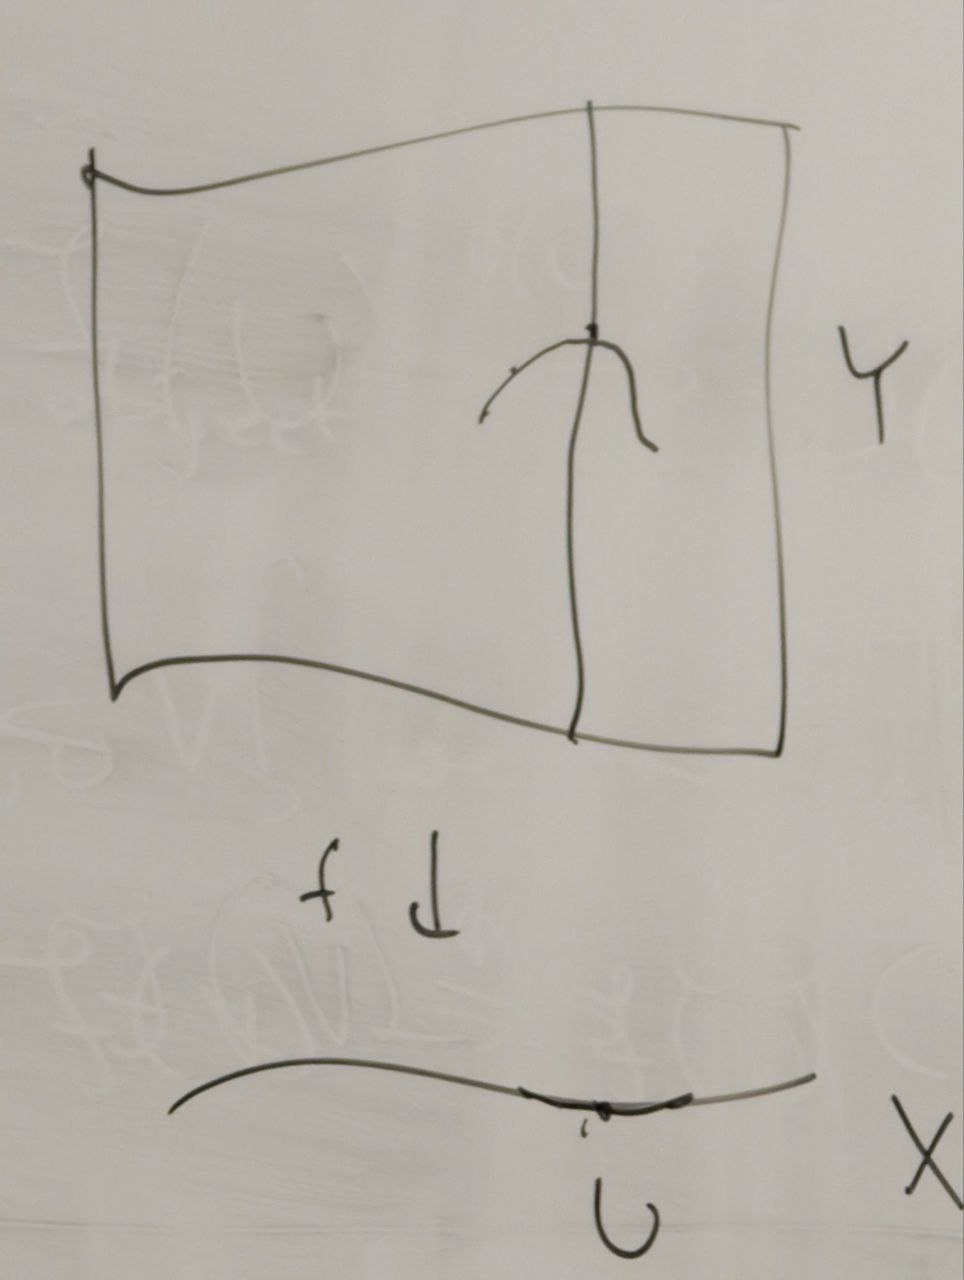
\includegraphics[width=0.4\textwidth]{img/section}
        \caption{}
    \end{figure}

    The \textit{stalk} of \(x\in X\) is \(\varinjlim_{U \ni x} \mathcal{F}(U)\).

    If \(\mathcal{F}\) is a presheaf of analytic functions on \(X = \mathbb{C}\), what is the stalk at \(x = 0\)?

    It is defined by the taylor series. So it contains power series with positive radius of convergence.

    Suppose \(U \subset X\) is open. Let \(U_\alpha\) be an open cover of \(U\). We also have \(\bigcup_{\alpha \in I} U_\alpha = U\).

    We have two obvious maps \(\prod_{\alpha \in I} \mathcal{F}(U)\) to \(\prod_{\beta ,\gamma \in I} \mathcal{F} (U_\beta \cap U_\gamma)\).

    \[
        \begin{tikzcd}
            \prod_{\alpha \in I} \mathcal{F}(U) \ar[r, bend left, "\phi : \alpha \mapsto \beta"] \ar[r, bend right, "\psi : \alpha \mapsto \gamma"] & \prod_{\beta, \gamma\in I} \mathcal{F}(U_\beta \cap U_\gamma)
        \end{tikzcd}
    \]

    Let's take a look into this. We have sections \((s_\alpha)_\{ \alpha \in I \} \mapsto (t_{\beta, \gamma})_{\beta, \gamma}\).

    \(\phi((s_\alpha))_{\beta,\gamma} = \operatorname{Res}_{U_\beta, U_\beta \cap U_\gamma} s_\beta \)
    
    \(\psi((s_\alpha))_{\beta ,\gamma} = \operatorname{Res}_{U_\gamma, U_\beta \cap U_\gamma} s_\gamma\).
    
    

    Thus we have:

    \[
        \begin{tikzcd}
            \mathcal{F}(U) \ar[r] & \prod_{\alpha \in I} \mathcal{F}(U) \ar[r, bend left, "\alpha \mapsto \beta"] \ar[r, bend right, "\alpha \mapsto \gamma"] & \prod_{\beta, \gamma\in I} \mathcal{F}(U_\beta \cap U_\gamma)
        \end{tikzcd}
    \]

    This diagram commutes.

    Let \(\mathcal{F}: \operatorname{Open}(X) \to \mathcal{C}\). If \(\Delta \in \operatorname{ob} \mathcal{C}\) then,

    \[
        \begin{tikzcd}
            \Delta \ar[d,dotted] \ar[rd] \\ \mathcal{F}(U) \ar[r] & \prod \mathcal{F}(U_\alpha) \ar[r, bend right] \ar[r, bend left] & \prod \mathcal{F} (U_\beta \cap U_\gamma)
        \end{tikzcd}
    \]

    If \(s_\alpha \in \mathcal{F}(U_\alpha)\) is a collection of sections so that \(\forall \beta ,\gamma\), \(s_\beta\) and \(s_\gamma\) agree on overlaps, i.e. \(\operatorname{Res}_{U_\beta, U_\beta \cap U_\gamma} s_\beta = \operatorname{Res}_{U_\gamma , U_\beta \cap U_\gamma} s_\gamma\) then \(\exists s\in \mathcal{F}(U)\) such that \(\operatorname{Res}_{U, U_\alpha} s = s_\alpha\) for all \(\alpha\).

    This is the sheaf axiom.

    Since there exists the empty product, we have to have a terminal object. But in our definition of the category of rings, we are excluding the zero ring so we don't have a final object in that category. But then we cannot define schemes. We need to modify some things.

    \subsection*{Presheaf which is not a Sheaf}

    We want to define sheaves. Consider the following example:

    Let \(X = \mathbb{R}\) and \(\mathcal{F} =\) sheaf of continuous functions \(X \to \mathbb{Z}\). Let \(\mathcal{G} =\) presheaf of constant \(\mathbb{Z}\)-valued functions on \(X\).

    Then, \(\mathcal{G}(U) = \mathbb{Z}\) for all \(U\neq \varnothing\).

    \(\mathcal{G}(\phi) = (0)\).

    \(\mathcal{F}\) agrees with \(\mathcal{G}\) on connected sets. But not necessarily on disconnected sets.

    \(\mathcal{G}\) is not a sheaf!

    What are the stalks of \(\mathcal{F}\) and \(\mathcal{G}\)?

    In both cases, the stalk at every point is \(\mathbb{Z}\).

    Furthermore, in the category of presheaves, there is a map \(\mathcal{G} \to \mathcal{F}\) in the sense that we have \(\mathcal{G}(U) \to \mathcal{F}(U)\) which is essentially the identity. On the stalks, this is an isomorphism.

    In general, if \(\mathcal{G}\) and \(\mathcal{F}\) are both presheaves on \(X\) and \(\phi: \mathcal{G} \to \mathcal{F}\) is a morphism of presheaves, then \(\forall x\in X\), \(\phi\) induces a map \(\phi_x\) sending stalks to stalks: \(\phi_x : \mathcal{G}_x \to \mathcal{F}_x\).

    \[
        \begin{tikzcd}
            \mathcal{F}(U) \ar[r] & \mathcal{F}(W) & \mathcal{F}(V) \ar[l] \\ \mathcal{G}(U) \ar[u] \ar[r] & \mathcal{G}(W) \ar[u] & \mathcal{G} (V) \ar[u] \ar[l]
        \end{tikzcd}
    \]

    is commutative.

    Note that, we can thus have two different presheaves with the same stalks. We don't want this, stalk should contain all the data of a sheaf.

    Slogan: A sheaf is a local object, i.e. determined by local data: stalks and \textit{compatibility of nearby stalks}.

    \section*{Wednesday, 9/10/2025}
    
    Let \(\mathcal{F}\) be a presheaf, \(U \subset X\) open. We can look at sections of \(X\) inside \(U\). Let \(\mathcal{F}_x\) be the stalk of \(\mathcal{F}\) at \(x\). We have:

    \[
        \mathcal{F}(U) \to \text{(compatible germs over \(U\))} \subset \prod_{x\in U} \mathcal{F}_x 
    \]

    \[
        s \mapsto (s_x)_{x\in U}
    \]

    Claim: if \(\mathcal{F}\) is a sheaf, this map is a bijection.

    Suppose sections \(s,t \in \mathcal{F}(U)\) and \(s_x = t_x\) for all \(x\in U\).

    Germs \(s_x\) and \(t_x\) are equal implies for all \(x\in X\) we can find an open set \(V_x \subset U\) containing \(x\) and a section \(r\in \mathcal{F}(V_x)\) such that \(s_x  = [(r,V_y)] = t_x\).
    
    Meaning, \(\operatorname{Res}_{U,V_x} s = r = \operatorname{Res}_{U, V_x} t\).

    Note that \(\bigcup_x V_x = U\). Sheaf axiom says that two sections on an open cover are the same. So, \(s=t\). This proves that the map is injective.

    Suppose we have \((s_x)_{x\in U}\) are compatible.

    For each \(x\), define \(V_x \ni x\) and \(\sigma_x \in \mathcal{F}(V_x)\), \(s_x = (\sigma_x)_x\). We want to glue together the \(\sigma_x\). We want the gluability part of the sheaf axiom.

    Claim: \(\forall x,y, \operatorname{Res}_{V_x, V_x \cap V_y} \sigma_x = \operatorname{Res}_{V_y, V_x \cap V_y} \sigma_y\).
    
    \(\forall x,y, \exists \sigma \in \mathcal{F}(U)\) such that \(\operatorname{Res}_{U,V_y} \sigma = \sigma_x \forall x\). So we're done. 

    \begin{definition}
        The \'etal\'e space \([\mathcal{F}]\) of a sheaf \(\mathcal{F}\) is the disjoint union of their stalks with the topology generated by

        \[
            \left\{ [(s,x)] \mid x\in U, s\in \mathcal{F}(U) \right\} 
        \]
    \end{definition}

    We then have a map \([\mathcal{F}] \to X\). Compatible germs map to open neighborhood.

    Now suppose we have \(X \xrightarrow{f} Y\). If \(\mathcal{F}\) is a sheaf we can define the \textit{pushforward of \(\mathcal{F}\) by \(f\)}.

    \[
        f_{\ast} (\mathcal{F})(U) = \mathcal{F}(f ^{-1} (U))
    \]

    Example: suppose \(X = \{ y \}\) and \(f\) is the inclusion map.

    Let \(c \in \operatorname{ob} \mathcal{C}\). Let \(\mathcal{F}_{y,c}=\) sheaf over \(y\) with value \(c\). \(f: \{ y \} \hookrightarrow y \in Y\).
    
    \[
        f_{\ast} \mathcal{F}_{y,c}(U) = \begin{dcases}
            c, &\text{ if } y\in U \\
            0, &\text{ if } y\notin U
        \end{dcases}
    \]

    \begin{definition}
        A \textit{ringed space} is a pair \((X, \mathcal{O}_X)\) where \(X\) is a topological space and \(\mathcal{O}_X\) is a sheaf of commutative rings on \(X\).
    \end{definition}

    Examples: 

    \begin{enumerate}[label=\arabic*)]
        \item \(X\) is a topological space, \(\mathcal{O}_X\) is the sheaf of continuous \(\mathbb{R}\)-valued functions.
        \item \(X\) is a smooth manifold, \(\mathcal{O}_X\) is the sheaf of smooth functions on \(X\).
        \item \(X\) is a Riemann surface, \(\mathcal{O}_X\) is the sheaf of analytic functions on \(X\).
    \end{enumerate}
    
    \begin{theorem}
        The category of presheaves of \(\begin{pmatrix}
            \text{abelian grps} \\
            \text{vector spaces} \\
            \text{etc}
        \end{pmatrix} \) forms an abelian categories.
    \end{theorem}

    To prove this, we need to be able to compute kernels, images, cokernels.

    Let \(\phi : \mathcal{F} \to \mathcal{G}\) be a morphism of presheaves. We \textit{do it by sections}:

    \((\ker \phi)(U) = \ker \mathcal{F}(U) \xrightarrow{\phi(U)} \mathcal{G}(U)\).

    \((\operatorname{im} \phi )(U) = \operatorname{im} \phi(U)\) 

    \((\operatorname{coker} \phi) (U) = \operatorname{coker} \phi(U)\)

    If \((X, \mathcal{O}_X)\) is a ringed space, we can define a presheaf \(\mathcal{F}\) of \(\mathcal{O}_X\)-modules to be a presheaf of abelian groups and structure of \(\mathcal{O}_X(U)\)-module on each \(\mathcal{F}(U)\) compatible with restriction maps.

    Example: Let \(E \to X\) be a vector bundle.

    Let \(\mathcal{O}_X\) be the sheaf of rings of continuous functions over \(X\) and \(\mathcal{F}\) be the sheaf of continuous sections of \(E \to X\).

    The category of sheaves is a full subcategory of the category of presheaves. This means, morphisms of sheaves are the same as morphism of presheaves which just happen to be sheaves.

    The category \(\operatorname{Ab}_X\) of sheaves of abelian groups is again an abelian category.

    \begin{lemma}
        If \(\phi : \mathcal{F} \to \mathcal{G}\) is a morphism of sheaves of abelian groups over \(X\), then the presheaf kernel of \(\mathcal{F} \to \mathcal{G}\) is a sheaf:

        \(\mathcal{H} (U) \coloneqq \ker \left(\mathcal{F}(U) \xrightarrow{\phi(U)} \mathcal{G}(U)\right)\) is a sheaf.
    \end{lemma}

    \begin{proof}
        Given an open cover \(U = \bigcup_{\alpha} U_\alpha\) and given \(h \in \mathcal{H} (U)\) such that \(\operatorname{Res}_{U,U_\alpha}(h) = 0\) for all \(\alpha\) we have \(h = 0\).

        Reason: \(\mathcal{H}(U) \subset \mathcal{F}(U)\) so we only need to check if \(h\) is \(0\) in \(\mathcal{F}(U)\) which follows from the sheaf axiom.

        Given \(h_\alpha \in \mathcal{H}(U_\alpha)\) such that \(\operatorname{Res}_{U_\alpha , U_\alpha \cap U_\beta} h_\alpha = \operatorname{Res}_{{U_\beta , U_\alpha \cap U_\beta}} h_\beta \forall \alpha ,\beta \) then \(\exists h \in \mathcal{H}(U) \in \ker \left( \mathcal{F}(U_\alpha) \xrightarrow{\phi(U_\alpha)} \mathcal{G}(U_\alpha) \right)\).

        \(\phi(U_\alpha \cap U_\beta) \left( \operatorname{Res}_{U_\alpha , U_\alpha \cap U_\beta} h_\alpha - \operatorname{Res}_{U_\beta , U_\alpha \cap U_\beta} h_\beta \right) = 0\) 

        We have \(\operatorname{Res}_{U_\alpha , U_\alpha \cap U_\beta} \phi(U_\alpha)(h_\alpha) = \operatorname{Res}_{U_\beta , U_\alpha \cap U_\beta} \phi(U_\beta) (h_\beta)\).

        \(h_\alpha \in \mathcal{F}(U_\alpha)\) which maps to \(0\) on \(\mathcal{G}(U_\alpha)\) 

        \(h_\beta \in \mathcal{F}(U_\beta)\) maps to \(0\) in \(\mathcal{G}(U_\beta)\).

        Then \(\operatorname{Res}_{U_\alpha , U_\alpha \cap U_\beta} h_\alpha = \operatorname{Res}_{U_\beta , U_\alpha \cap U_\beta} h_\beta\) 

        By gluability \(\exists h \in \mathcal{F}(U)\) such that \(\operatorname{Res}_{U,U_\alpha} h = h_\alpha\).

        Question: Does \(h\in \mathcal{H}\)? WTS: \(\phi(U)(h) = 0\).
        
        \(\operatorname{Res}_{U,U_\alpha} \phi(U) (h) = 0 \forall \alpha\).

    \end{proof}

    In general, gluability on \(\mathcal{F}\) and separability on \(\mathcal{G}\) implies gluability on \(\mathcal{H}\).

    \section*{Friday, 9/12/2025}
    
    If \(\mathcal{F}, \mathcal{G}\) are sheaves and \(\phi: \mathcal{F} \to \mathcal{G}\) is a morphism, then if we take image in the category of presheaves, then \(\operatorname{im} (\phi) (U) = \phi(U)(\mathcal{F}(U)) \subset \mathcal{G}(U)\).

    Then \(\operatorname{im} (\phi)\) is not a sheaf.

    For sheaves, we need a different notion of images!

    The separability axiom is fine: if \(f_1, f_2\in \operatorname{im} (\phi)(U)\) and \(U = \bigcup_\alpha U_\alpha\) and \(\forall \alpha : \operatorname{Res}_{U, U_\alpha}(f_1) = \operatorname{Res}_{U,U_\alpha}(f_2)\) then \(f_1 = f_2\).

    Problem is gluability.

    Suppose \(g_\alpha \in \operatorname{im} (\phi) (U_\alpha)\) and \(\forall \alpha ,\beta\) we have \(\operatorname{Res}_{U_\alpha, U_\alpha \cap U_\beta} g_\alpha  = \operatorname{Res}_{U_\beta, U_\alpha \cap U_\beta} g_\beta\).

    Can we find a \(g\in \operatorname{im} (\phi)(U)\) such that \(\operatorname{Res}_{U,U_\alpha} (g) = g_\alpha\)?

    Note that since \(g_\alpha \in \operatorname{im} (\phi)(U_\alpha)\), there exists \(f_\alpha\in \mathcal{F}(U_\alpha)\) such that \(\phi(U_\alpha) (f_\alpha) = g_\alpha\).

    We can do this gluing if \(\operatorname{Res}_{U_\alpha , U_\alpha \cap U_\beta} f_\alpha = \operatorname{Res}_{U_\beta , U_\alpha \cap U_\beta}\) for all \(\alpha , \beta\) by gluability of \(\mathcal{F}\). But we don't necessarily have that, we can only deduce that \(\operatorname{Res}_{U_\alpha , U_\alpha \cap U_\beta} f_\alpha - \operatorname{Res}_{U_\beta , U_\alpha \cap U_\beta} f_\beta\)  is in \(\ker \phi(U_\alpha \cap U_\beta)\).

    Thus, if we want an abelian category of sheaves, we want a different notion of image and cokernels.

    \begin{theorem}
        If \(\mathcal{F}, \mathcal{G}\) are sheaves and \(\phi : \mathcal{F} \to \mathcal{G}\) is a morphism of sheaves which is an isomorphism at the stalk level, then \(\phi\) is an isomorphism.

        Isomorphism at the stalk level: \(\phi: \mathcal{F} \to \mathcal{G}\) induces \(\phi_x: \mathcal{F}_x \to \mathcal{G}_x\) for each \(x\in X\). We want this to be an isomorphism.

        Slogan: A sheaf is determined by its stalks.
    \end{theorem}

    \begin{proof}

        Let \(U\) be any open subset of \(X\). We want \(\phi(U): \mathcal{F}(U) \to \mathcal{G}(U)\) to be an isomorphism.

        Suppose \(f_1, f_2\in \mathcal{F}(U)\) such that \(\phi(U)(f_1) = \phi(U)(f_2)\). Then \(\forall x\in U\), the germ of \(f_1\), which we write as \(f_{1,x}\) and the germ of \(f_2\), \(f_{2,x}\) map to the same germ, i.e. \(\phi(U)(f_1)_x = \phi(U)(f_2)_x\) in \(\mathcal{G}_x\). So, \(f_{1,x} = f_{2,x}\) for all \(x\in U\). Thus \(\exists U_x \subset U\) such that \(\operatorname{Res}_{U,U_x} f_1 = \operatorname{Res}_{U,U_x} f_2\).

        By separability, \(f_1 = f_2\).

        Now we prove gluability. Let \(g\in \mathcal{G}(U)\). \(\forall x\in U\) we have \(g_x = \phi_x(f_x)\) for some (unique) \(f_x \in \mathcal{F}_x\).

        Then \(\exists f_{U_x} \in \mathcal{F}(U_x)\) such that \(f_{U_x}\) represents \(f_x\) where \(U_x\) is a neighborhood of \(x\).

        Then \(\phi(U_x)(f_{U_x}) = g_{U_x}\) which has stalk \(g_x\). Then there exists \(U_x \supset V_x \ni x\) such that \(\phi(V_x)(\operatorname{Res}_{U_x, V_x}f_{U_x}) = \operatorname{Res}_{U,V_x}(g)\).
        
        Define \(f_{V_x}^{\prime} = \operatorname{Res}_{U_x, V_x} f_{U_x}\). Then, \(\phi(V_x)(f^{\prime} _{V_x}) = \operatorname{Res}_{U, V_x} (g)\).

        Claim: \(\{ f^{\prime}_{V_x} \}\) agree on overlaps.

        Proof: \(\forall x,y\in U\) we have \(\operatorname{Res}_{V_x, V_x\cap V_y} (f^{\prime} _{V_x}) = \operatorname{Res}_{V_y, V_x\cap V_y}(f^{\prime}_{V_y})\). This is true stalk by stalk and \(\mathcal{F}\) is a sheaf. By gluability we can find \(f^{\prime} \in \mathcal{F}(U)\) such that \(\operatorname{Res}_{U,V_x} f^{\prime} = f^{\prime} _{V_x}\) for all \(x\).

        Therefore, \(\phi(U)(f^{\prime})_x = g_x\) for all \(x\). \(\phi(U)(f^{\prime}) = g\).

    \end{proof}

    Given a presheaf \(\mathcal{F}\) there exists at most one sheaf \(\mathcal{G}\) and morphism \(\mathcal{F} \to \mathcal{G}\) which is an isomorphism of stalks at each \(x\). The process of finding such a \(\mathcal{G}\) is called \textit{sheafification}.

    \begin{definition}
        [Sheafification] Let \(\mathcal{F}\) be a presheaf. We define its sheafification \(\mathcal{F} ^{sh}\) in the following way:

        The stalks \(\mathcal{F}_x^{sh}\) are the same as \(\mathcal{F}_x\).

        Compatibility is the same.

        Let us be very specific about what sections are.

        \(\mathcal{F}^{sh} = \text{functions } U \to \coprod_{x\in U} \mathcal{F}_x\) such that each \(x\in U\) maps to \(f_x\in \mathcal{F}_x\) such that \(f_x\) are compatible as usual. 
    \end{definition}

    We need to check if \(\mathcal{F}^{sh}\) is actually a sheaf, and if there exists a map \(\mathcal{F} \to \mathcal{F}^{sh}\) which is an isomorphism at the stalk level.

    WTS: \(f_\alpha \in \mathcal{F}^{sh}(U_\alpha)\) and \(\forall \alpha ,\beta\) we have \(\operatorname{Res}_{U_\alpha , U_\alpha \cap U_\beta} (f_\alpha) = \operatorname{Res}_{U_\beta , U_\alpha \cap U_\beta}(f_\beta)\) then \(\exists ! f \in \mathcal{F}^{sh}(U)\).

    \(f_\alpha\) gives us a function \(U_\alpha \to \coprod_{x\in U_\alpha} \mathcal{F}_x\).
    
    \(f_\beta\) gives us a function \(U_\beta \to \coprod_{x\in U_\beta} f_x\).

    \(\forall x\in U_\alpha \cap U_\beta\) we have \(f_{\alpha, x} = f_{\beta , x}\).

    Define \(f_x = f_{\alpha , x}\) for some \(\alpha\) with \(x\in U_\alpha\).

    Now we need the map \(\mathcal{F} \to \mathcal{F}^{sh}\). Consider \(\mathcal{F}(U) \to \mathcal{F}^{sh}\) given by \(f \mapsto (x \mapsto f_x)\).
    
    We trivially have \(\mathcal{F}_x^{sh} = \mathcal{F}_x\): let \(s_x = [(s\in \mathcal{F}(U), x)]\). \(s\) defines compatible germs in a neighborhood of \(x\) therefore a section of \(\mathcal{F}_x^{sh}\) in a neighborhood of \(x\).

    \subsection*{Exponential Sequence for analytic functions on \(X = \mathbb{C} \setminus \{ 0 \}\)}

    Let \(\mathcal{O} =\) analytic functions [as additive group]

    \(\mathcal{O} ^\times =\) non-vanishing analytic functions [as multiplicative group]

    Let \(\underline{\mathbb{Z}}\) be sheaf of locally constant \(\mathbb{Z}\)-valued functions.

    We have the following:

    \[
        \begin{tikzcd}
            0 \ar[r] & \underline{\mathbb{Z}} \ar[r] & \mathcal{O} \ar[rr, "f \mapsto \exp(2 \pi i f)"] & & \mathcal{O}^\times \ar[r,"?"] & 0
        \end{tikzcd}
    \]

    Question: is this sequence exact?

    We can't take log uniquely in \(\mathcal{O}^\times\) so not for presheaves. But we can take log locally, so on the stalk level we can take log and thus this is a short exact sequence for sheaves!

    Slogan: Exactness for presheaves is determined on the section level, exactness for sheaves is determined on the stalk level.

    Let \(\phi : \mathcal{F} \to \mathcal{G}\) be a morphism of sheaves in an abelian category.

    \(\operatorname{im} (\phi)_{\text{sheaves}} = (\operatorname{im}(\phi)_{\text{presheaves}})^{sh}\)

    \(\operatorname{coker}(\phi)_{\text{sheaves}} = (\operatorname{coker}(\phi)_{\text{presheaves}})^{sh}\) 
    
    \begin{theorem}
        If \(\mathcal{F}\) is a presheaf, \(\mathcal{F}^{sh}\) is the universal sheaf admitting a map from \(\mathcal{F}\).
    \end{theorem}

    Thus, if \(\mathcal{F}\) is a presheaf and \(\mathcal{G}\) is a sheaf and we have \(\mathcal{F} \to \mathcal{G}\) we have a unique \(\mathcal{F}^{sh} \to \mathcal{G}\).
    
    \[
        \begin{tikzcd}
            \mathcal{F} \ar[r] \ar[rd] & \mathcal{F}^{sh} \ar[d, dotted] \\ & G
        \end{tikzcd}
    \]

    Sheafification is a functor. There is also a forgetful functor from sheaves to presheaves.

    Sheafification is the left adjoint of the forgetful functor.

    If \(\mathcal{F}\) is a presheaf and \(\mathcal{G}\) is a sheaf,

    \[
        \begin{tikzcd}
            \operatorname{Mor}_{\text{sheaves}} (\mathcal{F}^{sh}, \mathcal{G}) \ar[r, "\cong"] & \operatorname{Mor}_{\text{presheaves}} (\mathcal{F} , \mathcal{G}) 
        \end{tikzcd}
    \]

\end{document}